\documentclass[conference,10pt]{IEEEtran}
\usepackage{fontspec,xeCJK}
\setmainfont{texgyretermes-regular.otf}[BoldFont=texgyretermes-bold.otf,ItalicFont=texgyretermes-italic.otf,BoldItalicFont=texgyretermes-bolditalic.otf]
\setCJKmainfont{FandolSong-Regular.otf}[BoldFont=FandolSong-Bold.otf,ItalicFont=FandolKai-Regular.otf]
\setCJKsansfont{FandolHei-Regular.otf}[BoldFont=FandolHei-Bold.otf]
\usepackage{amsmath,amssymb,booktabs,graphicx,url,array}
\usepackage[hidelinks]{hyperref}
\renewcommand{\abstractname}{摘\ 要}
\renewcommand{\IEEEkeywordsname}{关键词}
\renewcommand{\refname}{参考文献}
\setlength{\emergencystretch}{1em}
\graphicspath{{figures/}}
\title{Augsburg多传感器融合与模态缺失鲁棒性实验\\MSH-Net复现与随机模态丢弃扩展}
\author{\IEEEauthorblockN{多传感器融合课程项目组}
\IEEEauthorblockA{公开匿名版\\Augsburg HSI + SAR + DSM}}

\IEEEoverridecommandlockouts
\IEEEaftertitletext{\noindent\begin{minipage}{\textwidth}
\small\normalfont
\textbf{贡献声明与排序}\quad 按署名顺序列示本次交付与答辩责任。\par\vspace{0.3em}
\begin{tabular}{@{}p{0.14\textwidth}@{\hspace{0.02\textwidth}}p{0.84\textwidth}@{}}
1\quad 成员A & 项目统筹、代码与环境复核、实验协议及最终材料整合。\\[0.2em]
2\quad 成员B & 数据与基线核查、缺失及噪声实验分析、图表与结果复核。\\[0.2em]
3\quad 成员C & 文献与论文对照、消融分析、演示与复现文档整理。
\end{tabular}
\end{minipage}\par
\vspace{0.8em}}
\begin{document}
\maketitle
\begin{abstract}
\normalfont\small\mdseries
面向传感器缺失条件下的遥感地物分类，本作业在Augsburg高光谱、合成孔径雷达与数字表面模型数据上，构建单模态、简单融合、跨模态知识蒸馏与随机模态丢弃特征融合的统一实验。使用608个训练点、153个验证点及77533个官方测试点，在24\,GB统一内存的Apple Silicon环境完成18个训练阶段和82个测试条件。完整模态教师的总体准确率达91.69\%，较最佳单模态基线提高2.41个百分点。随机模态丢弃扩展在仅保留SAR与DSM时达到82.27\%，较普通教师提高75.45个百分点；在仅保留HSI时达到91.12\%。噪声实验中，SAR学生在标准差0.10的扰动下较单模态基线提高11.45个百分点。结果表明，多源融合、缺失模式训练及跨模态蒸馏可在相应条件下发挥互补作用。报告结合消融、类别误差与原论文对照分析这些收益的适用条件，并提供逐样本结果、锁定环境及复现命令。
\end{abstract}
\begin{IEEEkeywords}
\normalfont\small\mdseries
多传感器融合，模态缺失，知识蒸馏，随机模态丢弃，遥感分类，可复现
\end{IEEEkeywords}

\section{问题背景与项目目标}
遥感地物分类可以同时利用光谱、散射和高度信息。高光谱影像（HSI）具有丰富的光谱通道，合成孔径雷达（SAR）提供与散射特性相关的观测，数字表面模型（DSM）描述地表高度结构。不同来源之间既有互补性，也存在分布、通道数和噪声特性的差异。多模态学习涉及表征、对齐、融合与协同学习等问题，早期与晚期融合只是其中的不同实现路径\cite{baltrusaitis2019}。多源基准及共享、特有特征学习研究为评估这种互补性提供了公开数据条件\cite{hong2021}。完整输入上的准确率无法回答部署时某一来源失效的问题，因此融合收益与缺失适应能力需要分开检验。

MSH-Net通过完整模态教师向单输入学生传递知识，并将学生与常规单模态网络的输出融合\cite{wei2023}。其核心动机是利用训练阶段存在而推理阶段缺失的信息。一般知识蒸馏通过教师的软输出指导学生\cite{hinton2015}；跨模态蒸馏进一步将这种指导用于传感器可用性不同的训练与测试场景，Garcia等在RGB与深度动作识别上研究了训练期多模态、测试期单模态的幻觉网络\cite{garcia2018}。教师只参与训练与蒸馏，最终部署模型仍可仅接收一种可用模态。该方案适合作为课程复现对象，但复现不应只比较运行是否成功，也应检查模型相对单模态基线是否有额外收益，以及收益是否依赖评价指标。

本作业围绕三个可检验问题展开：完整数据条件下，多模态特征融合是否优于单传感器与简单融合；当测试输入缺失时，专门训练的单输入网络是否优于直接对完整输入模型做零填充；蒸馏和输出融合是否在干净输入、噪声输入与各类别上都产生一致改善。为形成自己的课程技术改动，在相同多分支融合结构中引入样本级随机模态丢弃训练。该改动借鉴ModDrop的随机丢弃思想\cite{neverova2015}，并适配到本作业的三源分类流程，不作为新的学术算法提出。

项目交付包含技术报告、总结演示、公开代码仓库、数据获取脚本、小样本演示以及正式实验结果。正式评估范围为Augsburg三模态、训练seed为42的实验。其他模态组合的运行入口供后续复用，未列入本次结果；环境检查仅验证流程，不作为正式性能。

\section{数据、任务与评价协议}
\subsection{数据来源与模态}
Augsburg来自公开的S2FL基准\cite{hong2021,dataset}。对齐后的三种输入具有相同的$332\times485$空间尺寸：HSI含180个通道，SAR含4个特征通道，DSM含1个通道。DSM是高度表征而非普通可见光图像。本文将三者记为$\mathcal M=\{H,S,D\}$，任务是根据以待分类像素为中心的局部邻域，预测七类地物之一。图\ref{fig:data}显示三个来源的可视化，图像仅用于说明输入差异，不改变网络实际使用的通道。

\begin{figure*}[t]
\centering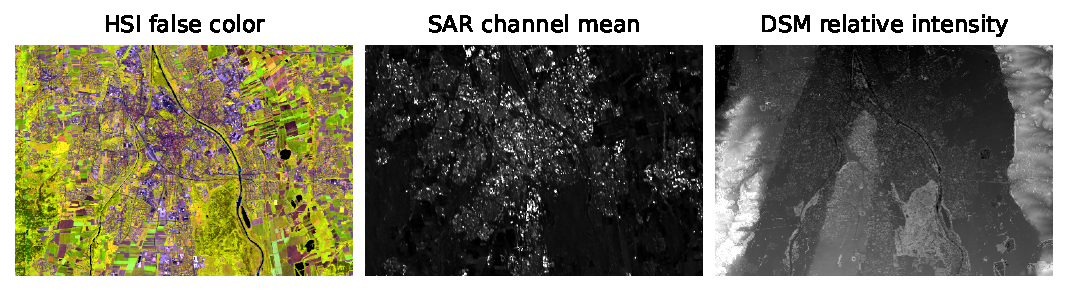
\includegraphics[width=.87\textwidth]{data_sources.pdf}
\caption{Augsburg输入来源。HSI为索引70、40、20（从0开始）通道的假彩色显示，SAR为四通道均值，DSM为相对强度。每幅图按1\%与99\%分位拉伸，仅影响显示；网络仍使用逐波段归一化的全部通道。}\label{fig:data}
\end{figure*}

官方标注包含761个训练点和77533个测试点。本文从官方训练点按类别分层抽取20\%作为内部验证集，固定划分seed为2026，得到608个训练点和153个验证点。表\ref{tab:data}列出各类别数量。所有方法使用相同划分，官方测试集在本次请求的模型训练与选择完成后才读取。该协议没有再使用训练与验证点进行全量重训，因此与论文使用761个训练点的设置不同。

\begin{table}[t]\centering\caption{类别与样本数量；测试类别顺序与原论文表II一致}\label{tab:data}
\begin{tabular}{lrrr}\toprule 类别 & 训练 & 验证 & 测试\\\midrule
森林&117&29&13361\\住宅区&211&53&30065\\工业区&17&4&3830\\低矮植被&198&50&26609\\园圃&41&11&523\\商业区&6&1&1638\\水体&18&5&1507\\\midrule 合计&608&153&77533\\\bottomrule\end{tabular}
\end{table}

\subsection{预处理与输入构造}
输入为$7\times7$邻域。每个模态按整幅场景逐波段进行最小值--最大值归一化，常量波段的分母置为1。边界坐标采用重复边界取样。该设置沿用作者预处理约定，利用了未标注场景的范围统计，不能称为仅由训练点估计的归一化。Augsburg测试HSI按需裁剪邻域，避免加载约4.54\,GB的展开测试矩阵。此前逐一比较了三模态各761个作者训练patch，float32最大绝对差为0，标签顺序也一致。

训练、验证中心索引没有重复，但随机点划分不具有空间隔离性。坐标审计发现153个验证点全部处于某个训练点的Chebyshev距离3以内，其中148个在距离1以内。因此其$7\times7$邻域均与训练邻域重叠。对具有空间依赖的数据，随机划分可能低估独立区域上的预测误差，空间分块是文献讨论的一种评价策略\cite{roberts2017}。本文将内部验证用于一致的模型选择，但不把接近100\%的验证准确率解释为空间独立区域的泛化能力。

\subsection{评价指标}
总体准确率OA是全部正确分类像素占比。类别平均准确率AA在本任务中取七类召回率的等权平均。设混淆矩阵为$C$，总样本数为$N$，有
\begin{equation}
 \mathrm{OA}=\frac{\sum_c C_{cc}}{N},\qquad
 \mathrm{AA}=\frac1{7}\sum_{c=1}^{7}\frac{C_{cc}}{\sum_j C_{cj}}.
\end{equation}
Kappa为$(p_o-p_e)/(1-p_e)$，其中$p_o=\mathrm{OA}$，$p_e$由预测和真实类别边际频率计算。OA、AA以百分数报告，差异用百分点表示；Kappa以0至1的量纲保存。论文表格Ka采用0至100显示，比较时统一换算。

\section{融合方法与课程扩展}
\subsection{单模态与简单融合基线}
单模态基线分别使用HSI、SAR或DSM，采用作者单分支网络和交叉熵训练。输入级简单融合将所有模态沿通道维拼接，再送入同类单分支网络。决策级简单融合分别训练各模态分类器，测试时对类别概率等权平均。完整模态教师采用作者的多分支跨模态特征融合网络。上述方法覆盖输入、特征和决策三个融合层次。Hong等系统比较了遥感中的多种融合架构及跨模态学习设置\cite{hong2021mdl}，为本作业从简单基线到多分支特征融合的比较提供了方法背景。

对于完整模态训练的模型，缺失输入在归一化空间置为全零，保持其他输入不变，不针对测试子集重新训练。概率平均基线也保留全部分支，缺失分支读取零输入，因此它不同于只平均可用分支的方案。此定义解释了其仅保留HSI时为何不能退化为HSI单模型的性能。

\subsection{JAD蒸馏与共享、特有信息融合}
完整模态教师输出logits $z_t$和特征$f_t$。单输入学生只接收可用模态$x_v$，输出$z_s,f_s$。教师在蒸馏阶段冻结，学生损失为
\begin{equation}
 L_s=L_{\rm CE}(z_s,y)+\alpha L_{\rm MMD}(f_s,f_t)
       +\beta T^2 D_{\rm KL}(p_t^T\Vert p_s^T),\label{eq:jad}
\end{equation}
其中$p^T=\mathrm{softmax}(z/T)$，温度$T=2$。MMD衡量再生核Hilbert空间中分布均值嵌入的差异\cite{gretton2012}。本作业通过多核高斯核匹配特征分布，不要求恢复缺失传感器的真实观测；KL匹配软化后的输出分布。HSI学生取$(\alpha,\beta)=(2,1)$，SAR和DSM学生取$(1,5)$，与论文三模态参数说明一致。

本地实现将MMD中显式的$N\times N\times d$距离展开改为平方范数与矩阵乘法，以降低统一内存占用；保留原核形式，并对带宽下界做数值保护。CPU float64下对原损失及梯度的等价性检查已通过。该优化改变中间计算的内存需求，不引入新的教师信息或标签。

最终MSH将JAD学生与对应常规单模态分支组合：
\begin{equation}
 z=(1-\eta)z_h+\eta z_n,\qquad \eta=\sigma(a).\label{eq:fuse}
\end{equation}
BatchNorm使用训练批次统计和推理期运行统计\cite{ioffe2015}。本阶段冻结两分支特征提取器及BatchNorm统计，仅训练分类头和标量$a$，使冻结分支的特征分布保持稳定。两分支都接收同一种可用模态，教师不进入部署检查点。每种可用模态分别训练学生及MSH，本文没有实现保留两个输入的MSH学生。式\eqref{eq:fuse}遵循论文单权重形式，但sigmoid约束与初始等权不等于作者发布代码中初始为1和0的两个自由权重，此差异在复现讨论中保留。

\subsection{随机模态丢弃特征融合扩展}
Dropout通过随机丢弃网络单元缓解共同适应\cite{srivastava2014}，ModDrop则将随机丢弃用于模态通道及其融合\cite{neverova2015}。本作业的技术改动保持教师的多分支特征融合结构，在训练输入上加入样本级模态掩码。设$m=(m_H,m_S,m_D)$，以概率0.5保留完整输入，以剩余概率均匀选一个模态置零，即每个单模态丢弃掩码的概率为$1/6$。目标为
\begin{equation}
 \min_\theta\ \mathbb E_{(x,y),m}
 L_{\rm CE}\big(F_\theta(m_Hx_H,m_Sx_S,m_Dx_D),y\big).\label{eq:drop}
\end{equation}
该实现称为ModDrop扩展。其融合发生于各模态编码后的特征层，训练改动让网络直接接触缺失条件，测试不需额外教师。它借鉴已有随机模态丢弃思想\cite{neverova2015}，本作业贡献是与公开三模态网络、缺失协议及Mac复现流程结合，而非提出原始ModDrop算法。训练只覆盖完整与缺一个模态，测试仍包括缺两个模态，这种掩码分布差异需要在分析中说明。

\section{实验设计与实现}
\subsection{正式训练设置}
实验使用macOS arm64、Python 3.11.14、PyTorch 2.5.1和MPS。依赖由uv锁定。训练batch为32，SGD学习率$10^{-3}$、动量0.9、weight decay为$10^{-3}$，采用5 epoch线性warmup和随后cosine衰减。教师、单模态、学生、损失消融和ModDrop各训练500 epoch，最终融合100 epoch。每阶段以验证OA优先、验证CE打破平局选取best，last保存模型、优化器与历史以支持epoch边界恢复。

运行seed为42，划分seed固定为2026。作者构造器内部保留固定初始化seed，本地阶段按实验名与运行seed设定训练随机顺序。因此即使后续增加运行seed，也不能自动称为不同独立随机初始化。本批没有运行seed43和44的正式证据，不报告跨seed标准差、显著性或置信区间。

\subsection{实验矩阵}
核心实验包含三种单模态基线、输入拼接、概率平均、教师、三个JAD学生和三个MSH模型。拼接、平均和教师均测试七个非空输入子集，其余方法测试对应的单输入条件，共30条核心记录。扩展包含ModDrop的七种输入、六个KL-only或MMD-only学生、三个测试时固定$\eta=0.5$的干预，以及四类单输入方法在三档非零噪声下的36条记录，总计82个测试条件、18个独立训练阶段。

KL-only将式\eqref{eq:jad}的$\alpha$置零，MMD-only将$\beta$置零，其余配置保持对应设定。它们是学生级损失对照，没有再分别训练最终融合网络。不同实验名对应不同训练批次顺序，因此本次单seed消融提供趋势证据，不构成严格控制批次随机性的因果结论。固定$\eta$实验复用已有分类头，只在测试时改权重，不能替代从头固定权重训练。

\subsection{缺失与噪声量化}
三模态完整输入、三个缺一模态组合和三个缺两模态组合共同覆盖七种非空输入。噪声实验向可用的归一化输入加入独立高斯噪声，标准差为0.05、0.10、0.20，并截断到$[0,1]$。相同形状输入使用固定噪声实现，以便对照。该扰动不等同于实际传感器经标定后的误差分布，也不把标准差0.2解释为真实仪器20\%噪声。没有训练噪声增强，也没有噪声随机重复，因此结论限定于当前扰动实现。

\section{实验结果与分析}
\subsection{完整模态与单输入主结果}
表\ref{tab:main}列出主要干净输入结果。教师完整模态OA为91.69\%，比HSI单模态89.29\%高2.41个百分点，支持多源信息的互补价值。但输入拼接已经达到91.54\%，仅比教师低0.15个百分点，且AA为68.20\%，高于教师66.78\%。这说明在当前协议下，复杂特征融合没有展示相对简单拼接的明确全面优势。概率等权平均OA为88.85\%，低于HSI基线，说明引入较弱分支不保证改善整体分类。

\begin{table}[t]\centering\caption{主要干净输入结果；TEACHER、MODDROP、CONCAT、MEAN使用完整输入，其余使用名称所示单输入}\label{tab:main}\small\begin{tabular}{lrrr}
\toprule
方法/输入 & OA (\%) & AA (\%) & Kappa \\
SINGLE-HSI & 89.29 & 64.94 & 0.8458 \\
SINGLE-SAR & 81.18 & 43.62 & 0.7234 \\
SINGLE-DSM & 74.69 & 43.10 & 0.6278 \\
EARLY-CONCAT & 91.54 & 68.20 & 0.8782 \\
LATE-MEAN & 88.85 & 53.71 & 0.8346 \\
TEACHER & 91.69 & 66.78 & 0.8802 \\
JAD-HSI & 89.38 & 66.75 & 0.8480 \\
MSH-HSI & 89.59 & 66.25 & 0.8506 \\
JAD-SAR & 78.67 & 42.31 & 0.6870 \\
MSH-SAR & 80.48 & 43.07 & 0.7127 \\
JAD-DSM & 74.24 & 38.56 & 0.6177 \\
MSH-DSM & 75.41 & 39.98 & 0.6344 \\
MODDROP & 91.91 & 65.64 & 0.8833 \\
\bottomrule
\end{tabular}
\end{table}

MSH仅保留HSI时OA为89.59\%，比基线高0.30个百分点，AA由64.94\%增至66.25\%。JAD学生AA为66.75\%，反而高于最终MSH，表明输出融合在提高一点总体正确率的同时，也可能改变类别间权衡。仅SAR时，JAD的OA降至78.67\%，低于基线81.18\%；最终MSH回升到80.48\%，但仍低0.70个百分点。仅DSM时，MSH的OA比基线高0.72个百分点，AA却由43.10\%降至39.98\%。不能用OA的单项提高概括其全部表现。

\subsection{普通融合模型在缺失输入下的退化}
表\ref{tab:missing}展示固定完整输入训练模型的七种测试条件。教师仅保留HSI、SAR、DSM时OA分别为42.85\%、5.97\%、9.40\%，明显低于专门训练的对应单输入模型。该现象与论文所讨论的缺失分布偏移方向一致。但普通单模态基线也已经避免崩溃，因此“MSH高于零填充教师”不能独自证明蒸馏的额外价值。

\begin{table}[t]\centering\caption{不同可用输入下的OA（\%）；缺失输入全零填充}\label{tab:missing}\small\begin{tabular}{lrrrr}
\toprule
保留输入 & 拼接 & 平均 & 教师 & ModDrop \\
HSI+SAR+DSM & 91.54 & 88.85 & 91.69 & 91.91 \\
HSI+SAR & 64.79 & 87.38 & 83.25 & 91.69 \\
HSI+DSM & 83.62 & 87.71 & 55.65 & 91.41 \\
SAR+DSM & 2.87 & 83.97 & 6.82 & 82.27 \\
HSI & 40.42 & 34.32 & 42.85 & 91.12 \\
SAR & 2.37 & 68.94 & 5.97 & 69.51 \\
DSM & 2.76 & 36.65 & 9.40 & 49.29 \\
\bottomrule
\end{tabular}
\end{table}

教师保留HSI+SAR时OA83.25\%，保留HSI+DSM时55.65\%，保留SAR+DSM时6.82\%。简单拼接在相应条件下的排序不同，说明缺失性能反映训练后模型依赖以及输入分布变化，不能直接当作传感器固有重要性的排序。概率平均仅HSI时OA34.32\%、AA14.29\%、Kappa为0，预测退化为同一类；此处两个读零输入的分支仍参与平均，与运行single-HSI并不矛盾。

\subsection{随机模态丢弃扩展的收益与边界}
ModDrop完整输入OA为91.91\%，比普通教师高0.22个百分点，AA却低1.13个百分点。其主要收益出现在缺失条件：HSI+DSM由55.65\%提高至91.41\%，SAR+DSM由6.82\%提高至82.27\%，仅HSI由42.85\%提高至91.12\%。训练时引入缺失模式可以显著缓解普通教师的分布偏移，这构成本作业扩展的实证结果。

仅HSI时ModDrop的OA高于MSH约1.53个百分点，但AA63.61\%低于MSH66.25\%。仅SAR和仅DSM时，ModDrop的69.51\%和49.29\%仍低于相应单模态与MSH。其训练只丢一个模态，缺两个的条件没有直接覆盖，这是可能影响结果的机制之一，尚不能仅凭观测确定为唯一原因。

\begin{figure*}[t]\centering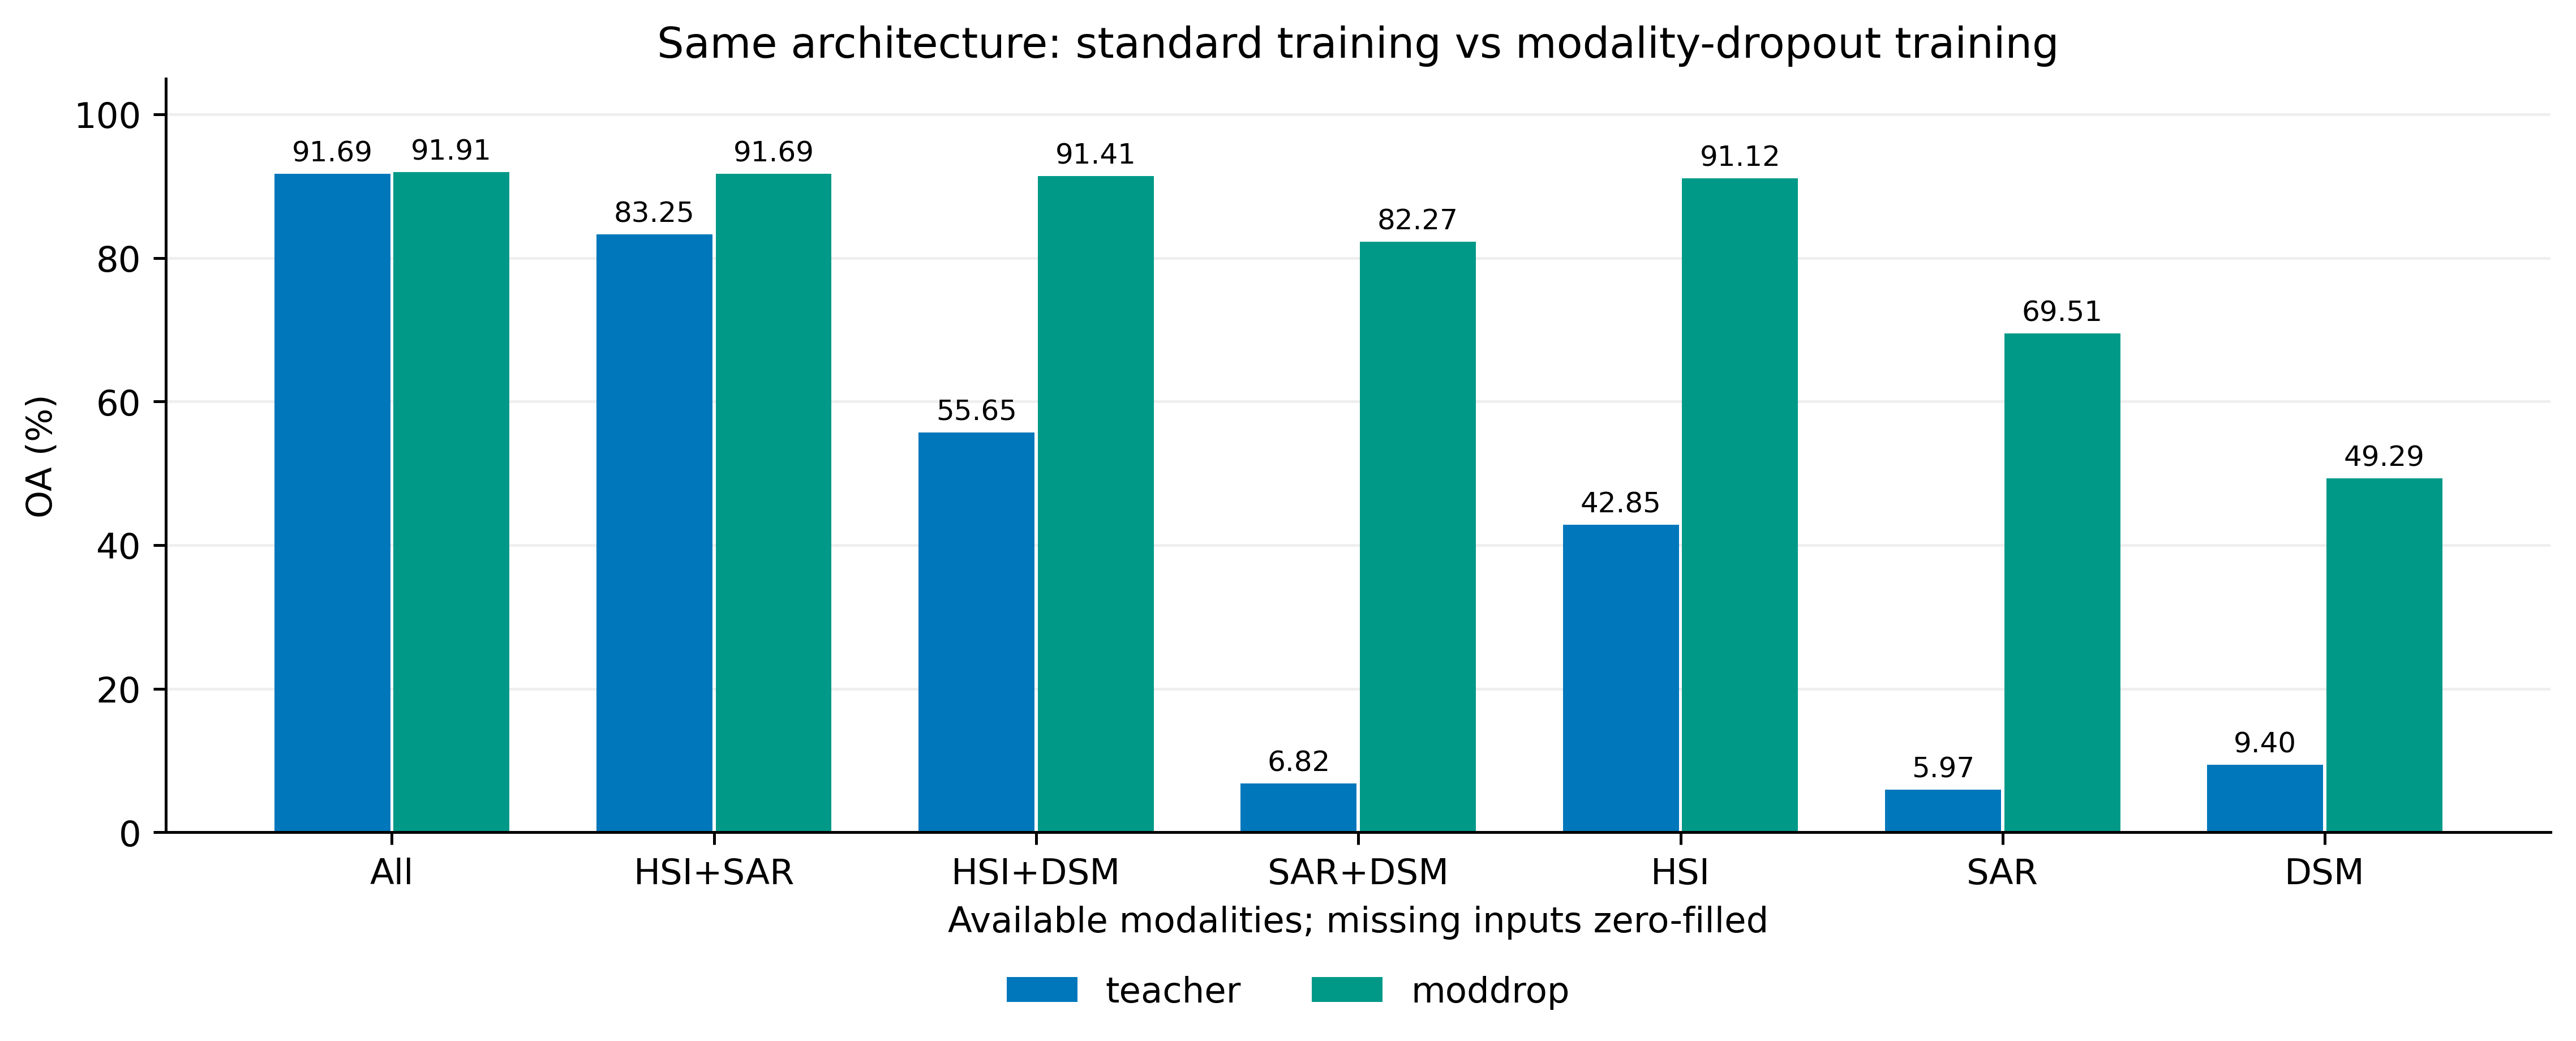
\includegraphics[width=.88\textwidth]{fig2_moddrop_missing.png}
\caption{相同结构的普通教师与随机模态丢弃扩展。在多种缺失条件下扩展取得更高OA，但对仅SAR/DSM仍不及对应单模态训练。}\label{fig:drop}\end{figure*}

\subsection{蒸馏损失消融}
表\ref{tab:ablation}显示联合MMD与KL没有在所有模态上优于单项。HSI的MMD-only OA为89.41\%，略高于JAD89.38\%，但JAD的AA66.75\%高于MMD-only65.09\%。SAR的MMD-only获得81.25\% OA和44.56\% AA，略优于CE基线，而JAD降到78.67\%和42.31\%。DSM的KL-only下降尤为明显，OA为71.52\%，其余蒸馏学生的AA也低于CE。当前结果提示输出蒸馏可能参与干净精度的负迁移，但教师质量、优化过程和阶段随机顺序也可能影响结果，不能作单一原因归结。

\begin{table}[!t]\centering\caption{学生损失消融的OA（\%）；MSH另含最终融合。各阶段仅一个训练seed，且训练顺序不同}\label{tab:ablation}\begin{tabular}{lrrrrr}
\toprule
输入 & CE & CE+KL & CE+MMD & JAD & MSH \\
HSI & 89.29 & 89.30 & 89.41 & 89.38 & 89.59 \\
SAR & 81.18 & 80.56 & 81.25 & 78.67 & 80.48 \\
DSM & 74.69 & 71.52 & 74.49 & 74.24 & 75.41 \\
\bottomrule
\end{tabular}
\end{table}

\subsection{噪声鲁棒性与干净精度的权衡}
图\ref{fig:noise}给出噪声曲线。HSI在标准差0.05时，JAD为75.10\%、MSH为69.14\%，高于基线59.46\%；标准差0.20时则降至8.63\%和11.18\%，低于基线12.89\%。这说明轻噪声收益不能推广为全部噪声强度下的优势。

SAR表现出不同权衡：JAD干净输入OA低于基线，但标准差0.10时为63.41\%，高于基线51.96\%共11.45个百分点；标准差0.20时54.80\%对42.83\%，高11.97个百分点，AA也更高。最终MSH在这些噪声条件下介于学生与基线之间。DSM的MSH在三档噪声下OA比基线高约0.48、1.28、0.93个百分点，AA却分别低约1.06、1.03、1.19个百分点，类别平均表现仍是其弱点。

\begin{figure*}[t]\centering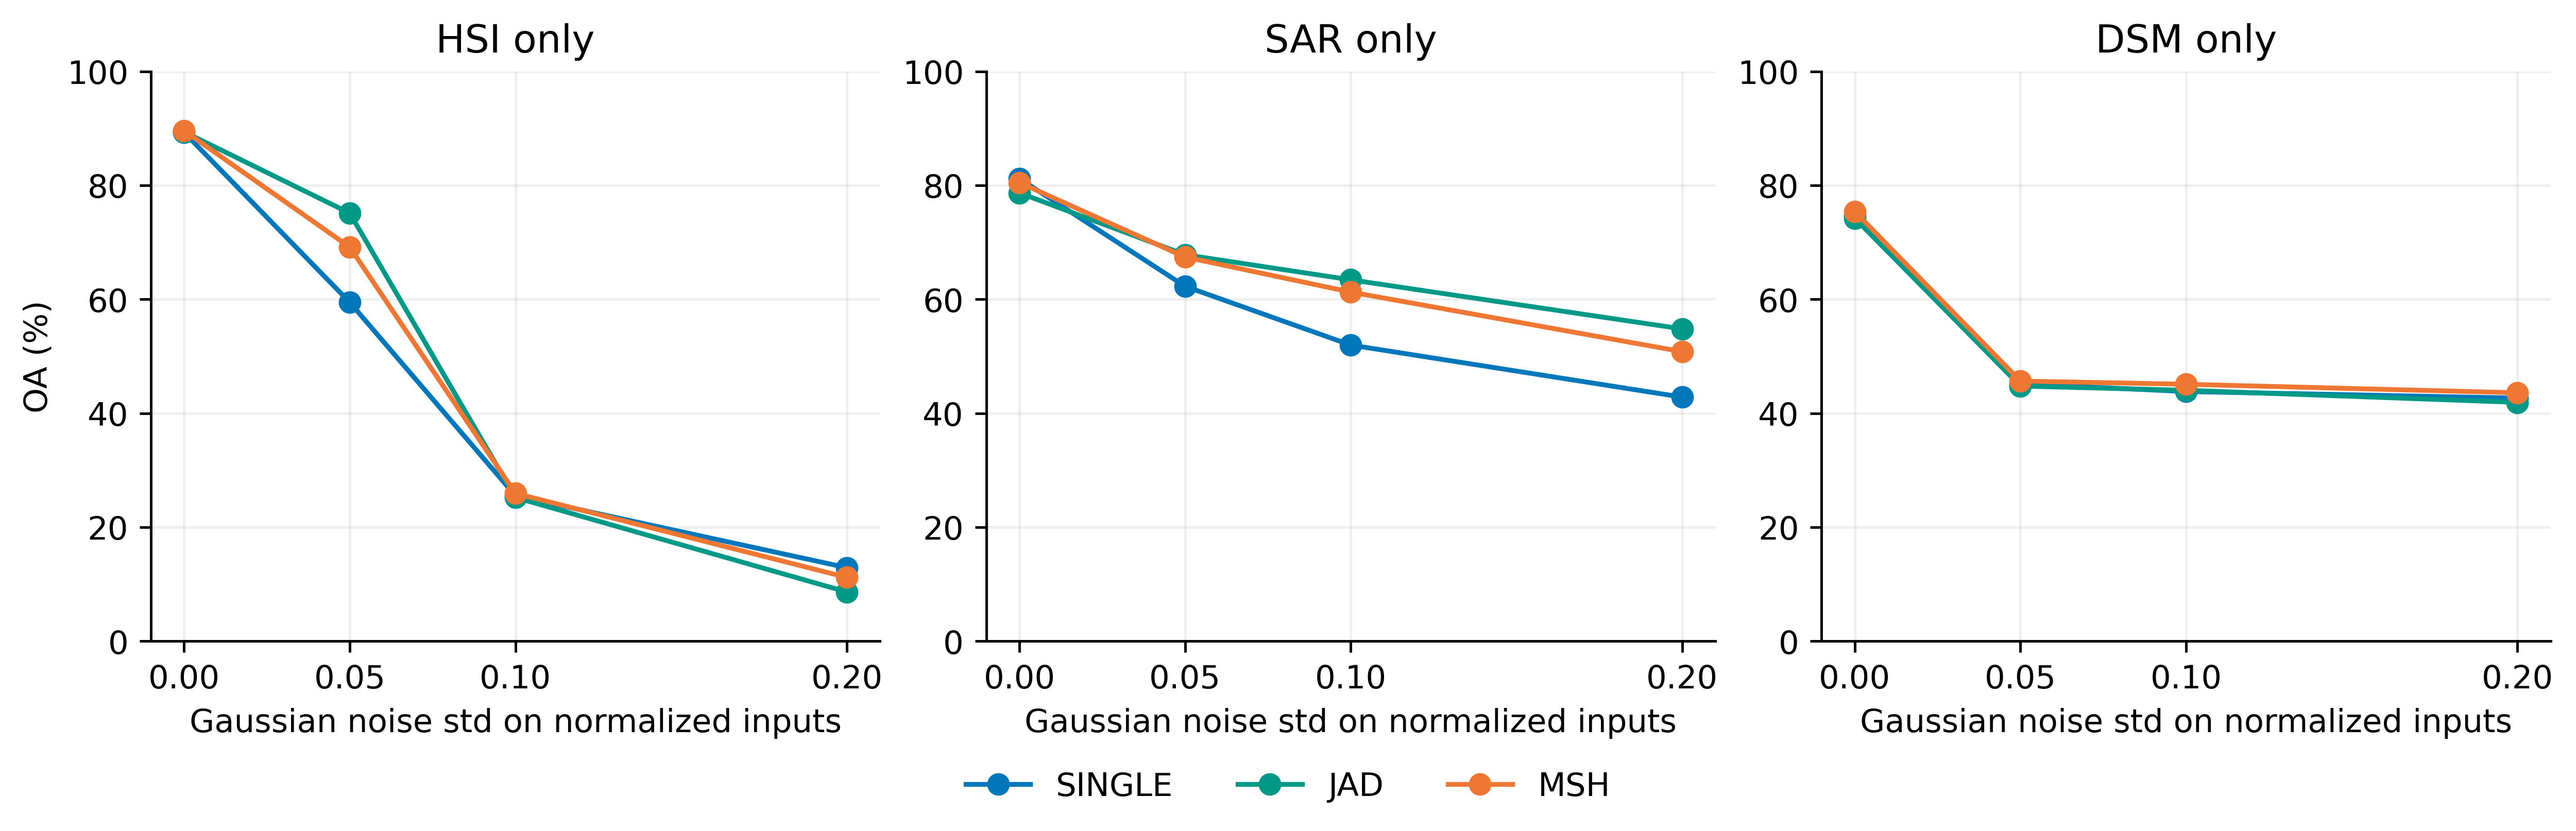
\includegraphics[width=.96\textwidth]{fig3_noise_robustness.png}
\caption{单可用模态的高斯噪声实验。横轴为归一化输入上的噪声标准差，纵轴为OA。所有曲线使用同一官方测试点，未进行噪声训练。}\label{fig:noise}\end{figure*}

\subsection{融合权重与类别误差}
三个MSH均在融合epoch=1选中best，其$\eta$分别约0.499999、0.499991、0.499978。将测试权重强制设为0.5，干净输入的三组预测完全不变；十二个干净/噪声对照中，只有SAR标准差0.05时改变一个像素的预测。最后epoch的权重确实有更新，因此不能说没有梯度；但保存用于测试的模型没有显示学习$\eta$相对近似等权融合的实质收益。该测试干预仍不足以替代固定权重从头训练的对照。

测试集中森林、住宅区和低矮植被占90.33\%，OA主要受这三类影响。商业区仅有6个训练点与1个验证点，教师召回率只有2.44\%，MSH-HSI为11.11\%，低于HSI基线14.41\%。MSH-DSM在住宅区召回率上升约3.92个百分点，却在园圃和工业区分别下降约17.59和6.19个百分点，解释了OA提高而AA下降。图\ref{fig:maps}给出测试标注位置上的空间结果，未对未标注像素进行补画或平滑。

\begin{figure*}[t]\centering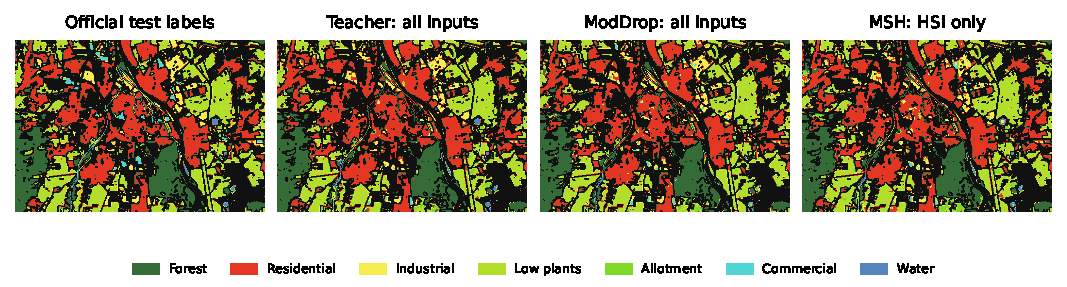
\includegraphics[width=.98\textwidth]{test_maps.pdf}
\caption{官方测试位置的标签与预测。黑色表示非官方测试标注位置，色彩依次对应七类地物；所有方法显示相同像素集合，未用后处理掩盖误差。}\label{fig:maps}\end{figure*}

\section{论文对照、可比性与局限}
\subsection{与原论文表VI的数值关系}
表\ref{tab:paper}统一使用原论文表VI，而非混用正文中不一致的数值。三个MSH输入的OA比论文分别低3.40、3.03、6.20个百分点。单模态基线已经偏低，但在基线之上的MSH额外增益也不足：论文HSI/SAR/DSM的OA增益为2.08、0.83、3.49个百分点，本地为0.30、$-$0.70、0.72个百分点。该对照同时呈现本地改善及其与论文结果的幅度差异。

\begin{table*}[t]\centering\caption{与原论文表VI的对照；差值为本地减论文，单位为百分点。两者训练协议不同}\label{tab:paper}\small\begin{tabular}{lrrrrrr}
\toprule
方法 & 论文OA & 本地OA & 差值 & 论文AA & 本地AA & 差值 \\
SINGLE-HSI & 90.91 & 89.29 & -1.62 & 65.32 & 64.94 & -0.38 \\
SINGLE-SAR & 82.68 & 81.18 & -1.50 & 46.12 & 43.62 & -2.50 \\
SINGLE-DSM & 78.12 & 74.69 & -3.43 & 41.96 & 43.10 & +1.14 \\
TEACHER & 93.31 & 91.69 & -1.62 & 63.85 & 66.78 & +2.93 \\
MSH-HSI & 92.99 & 89.59 & -3.40 & 66.86 & 66.25 & -0.61 \\
MSH-SAR & 83.51 & 80.48 & -3.03 & 44.11 & 43.07 & -1.04 \\
MSH-DSM & 81.61 & 75.41 & -6.20 & 43.60 & 39.98 & -3.62 \\
\bottomrule
\end{tabular}
\end{table*}

HSI改善方向与论文一致，但幅度较小。SAR的OA变化方向相反；DSM虽都有OA改善，论文AA提高1.64个百分点，本地下降3.12个百分点。论文的SAR AA本身也低于其单模态基线，所以不应将原文概括成所有模态、所有指标全面提高。本地实验展示了完整模态融合的互补收益，以及针对缺失条件训练的实际价值；MSH在HSI与DSM上的OA改善与论文方向一致。各模态的改善幅度和类别表现存在差异，应结合训练协议解释。

论文三模态正文把DSM与SAR的MSH OA写为81.86\%和83.35\%，表VI则为81.61\%和83.51\%。本文以视觉核对后的表格为准并重新计算差值，不自行挑选更接近本地的版本。论文表VII的蒸馏消融发生于Houston HSI+LiDAR，且比较对象不同，不能直接作为当前Augsburg学生消融的数值目标。ModDrop和本次高斯噪声扫描也不是表VI给出的实验，本文将其作为课程扩展的独立实证结果。

\subsection{已确认的协议差异}
训练点由761减为608，随机翻转增强未在当前正式入口实现，融合初始权重及约束也未完全对齐发布代码。论文正文采用三次运行平均，本地目前只有一个seed。作者发布脚本每epoch在名为test\_loader的官方测试分区上更新best，本地改用独立内部验证并在训练后评估官方测试。这些差异改变了训练与选择过程，不能视为等同设置。

本地主要训练阶段已完成500 epoch，训练loss大幅下降，不能简单归因为只训练了几步。缺少翻转是当前实现尚未对齐论文的一项，而非经消融证明可以忽略的选择。MPS和CPU均通过环境与反向传播检查，但现有数据没有分解平台数值差异与协议差异，因此不把所有精度差距归因于Mac。跨平台运行验证与论文表格对照分别用于检查工程可执行性和实验条件的可比性。

\subsection{空间验证与统计解释边界}
内部验证集较小且邻域重叠，一个验证点改变OA约0.65个百分点，商业区仅有一个验证点，使模型选择对微小差异和小类表现不敏感。报告披露这些局限，不将高验证OA作为独立泛化证据。不同损失阶段的训练顺序不同、噪声只使用固定随机实现，也限制了消融和鲁棒性结论的推广。后续应预先定义更严格的空间划分和配对随机过程，在不反复利用测试集选择的条件下检验改进。

\section{可复现实现与交付}
\subsection{代码、环境与数据}
代码仓库为\url{https://github.com/libo-zhu/sense-course}，提供作者网络与MIT许可证、上游commit、Mac适配、训练推理入口及结果审计脚本。\texttt{uv.lock}锁定依赖；运行\texttt{uv sync --locked}安装环境，数据由\texttt{scripts/prepare\_data.py}从公开来源下载。原始数据及原论文PDF不重新上传，避免把第三方内容混入公开代码。

\texttt{mac\_demo.py}用真实数据验证教师、学生、融合、缺失推理及检查点重载；默认每阶段三个更新，仅作流程检查。\texttt{run\_experiments.py}负责正式训练，支持自动依赖、epoch边界恢复和仅评估。完整命令在README与提交说明中给出，避免双栏长命令影响复制。

\subsection{结果追溯与Mac适配}
正式结果按组合与seed保存，\texttt{models/}提供检查点和历史，\texttt{evaluation/}提供指标、逐样本预测与混淆矩阵。混淆矩阵行是真实类、列是预测类，类别从0编码。分析脚本逐一复算82个条件的OA、AA、Kappa并核对原始TestImage标签列序；报告、PPT与CSV均使用这批正式结果。

设备显式选择MPS或CPU，结合MMD距离优化和测试邻域按需裁剪控制存储。真实数据demo的峰值进程RSS约1.34\,GiB；完整正式实验已在24\,GB统一内存设备上完成，但未单独测量完整训练峰值内存。CPU及原生MPS短程检查、冻结状态断言、独立权重推理和CPU恢复一致性检查均已通过。部署检查点只含对应单输入模型参数，教师不进入推理流程。

\section{结论}
本作业在Augsburg三模态地物分类上完成了从单传感器、简单融合到知识蒸馏和缺失适配扩展的可复现实验。完整模态教师OA达到91.69\%，较最佳单模态提高2.41个百分点；随机模态丢弃在SAR+DSM条件下达到82.27\%，体现了面向缺失模式训练的实际收益。MSH在HSI与DSM上的OA有所提高，SAR学生在中高强度噪声下表现出较强鲁棒性。这些结果为根据输入条件选择融合和蒸馏策略提供了实验依据。

论文表VI与本地结果的逐项对照提供了进一步优化的方向：对齐训练点数量与数据增强，完善融合参数和模型选择，并采用空间分块及配对多次实验评估稳定性。后续可扩展随机掩码分布以覆盖仅SAR或仅DSM的训练条件，并结合类别平衡方法改善小类表现。当前结论限定于已记录的单次运行、数据划分及扰动条件；完整数值与协议差异在正文和代码中保留，便于继续检验和扩展。

\IEEEtriggeratref{6}
\bibliographystyle{IEEEtran}
\bibliography{references}
\end{document}
